\usepackage{}\documentclass[final, dvipsnames, authoryear,12pt]{elsarticle}
\setcounter{page}{0} \renewcommand{\baselinestretch}{1.0}
\usepackage[utf8]{inputenc}
\usepackage{subfiles}
\usepackage{todonotes}
\usepackage[left=3cm, right=3cm, top=3cm]{geometry} 

\usepackage{epsfig,amssymb,calc,float,longtable,natbib,rotating,url, grffile, supertabular, subfig}

\setlength{\parindent}{0em}
\setlength{\parskip}{1em}

\usepackage{color}
\DeclareUnicodeCharacter{2212}{-}
\usepackage{blindtext}
\usepackage{mathtools}
\usepackage{mdframed}
\usepackage{graphicx}
\usepackage{caption}
\usepackage{subcaption}
\usepackage{enumerate}
\usepackage{hyphenat}
\usepackage[english]{babel}
\usepackage{colortbl}
\usepackage{amsmath}
\usepackage{booktabs}
\usepackage{multirow}
\usepackage{multicol}
\usepackage{makecell}

\usepackage{changepage}
\usepackage{soul}
%font types
\usepackage{tgcursor}
\usepackage{courier}

\usepackage{tabularx}
\usepackage{tabulary}
\usepackage{threeparttable}
\usepackage{lscape}

\usepackage{bigstrut}
\usepackage{filecontents}
\usepackage{hhline}


\begin{document}


\begin{frontmatter}
\title{Global Value Chain localisation and firms competitiveness: Lessons from the Central European Supplier Survey}






\author[gb]{G\'{a}bor B\'{e}k\'{e}s}
\author[mk]{Miklós Koren}
\author[bm]{Balázs Muraközy\corref{cor1}}
\author[at]{Álmos Telegdy}
 \address[gb]{Central European University, Institute of Economics and CEPR}
 \address[mk]{Central European University, Institute of Economics and CEPR}
 \address[bm]{University of Liverpool, Institute of Economics }
 \address[at]{National Bank of Hungary}
 
 
\cortext[cor1]{Corresponding author: Balázs Muraközy, University of Liverpool Management School, Chatham St, Liverpool L69 7ZH United Kingdom} 

\cortext[cor2]{The authors gratefully acknowledge funding from the European Research Council (ERC Starting Grant agreement number 313164) and  the European Union’s Horizon 2020 research and innovation programme (under grant agreement No 822390, the Microprod project). We thank Kinga Ritter, Imola Csóka, Gergely Kiss, Krisztián Fekete and András Vereckei for excellent research assistance.}



\begin{abstract}

    
       \vspace{2mm} 
   
   \textbf{keywords:} supplier-buyer relationships, supplier survey, relationship formation, innovation, data handling and cleaning 
   
    \vspace{2mm}
    
   \textbf{JEL-codes:} C83, D22, D23 
\end{abstract}


\end{frontmatter}
%\maketitle

%%%%%%%%%%%%%%%%%%%%%%%%%%%%%%%%%%%%%%%
\section{Introduction}
%%%%%%%%%%%%%%%%%%%%%%%%%%%%%%%%%%%%%%%

The new wave of globalization in the 1990s brought about the formation of Global Value Chains (GVCs). These are companies linked by ownership and trade connections and are among the most important production structures of the global economy. The scale and importance of GVCs has multiplied during the last three decades.\footnote{\cite{mckinsey2019gvc}, for example, identify 23 GVCs and find that they account for 69 percent of global output and 96 percent of international trade.} Linking their countries' companies to GVCs is also high on the agenda of governments, as the integration into the production chains is considered to be among the most effective ways of improving competitiveness of firms.





This approach raised a number of methodological dilemmas, but at the same time revealed novel patterns about relationship formation and the operation of relationships. Even though this approach has a number of shortcomings, we think that methodologies combining qualitative data with financial information are a promising approach for understanding GVCs and the importance of buyer-supplier relationships in firm performance. The aim of this paper is to describe our approach in detail, compare it to other approaches used in the literature and to describe a number of relevant patterns identified from the data. 

In what follows, Section \ref{sec: approach} describes and compares the various approaches used in the literature to understand buyer-supplier relationships. Section \ref{sec:survey} details our approach and the process of conducting the survey. Section \ref{sec:question} describes the main variables from the questionnaire while Section \ref{sec:data_handling} discusses how we cleaned and handled the data. Section \ref{sec:desc} describes the first results from the survey while \ref{sec:conclusions} concludes.  

%%%%%%%%%%%%%%%%%%%%%%%%%%%%%%%%%%%%%%%
\section{Approaches to understand GVCs and supplier-buyer relationships} 
\label{sec: approach}
%%%%%%%%%%%%%%%%%%%%%%%%%%%%%%%%%%%%%%%

\subsection{Existing approaches and results}

To understand the importance of GVCs and their effect on countries, early research relied on industry-level input-output tables, constructed from international trade data \citep{johnson2012accounting, hummels2001nature}. The main purpose of the use of such data were to (1) measure flows of trade between industries and countries and (2) compute the share of value added in gross exports. The data were also used to understand the propagation and amplification of small shocks in the economy \citep{acemoglu2016networks}. A key finding based on aggregate data is that intermediate inputs played an ever growing role in international trade since the 1970s, increasing abruptly in the 1990s. 



An emerging literature studies business linkages and their effects on firm behavior at the firm level. These papers rely on two types of datasets: those of administrative origin and surveys. \footnote{A common feature of all these data are that information on linkages and on firm performance (in form of balance sheet and income statement) are from different sources, and the performance data usually is of administrative origin.} 

In Europe, administrative data on buyer-supplier links are mainly derived from VAT filings. \cite{dhyne2015belgian} describe a dataset that covers Belgian companies. In addition to its extensive coverage (about 400 thousand firms), the data also follows firms for the extended period of 11 years. Papers using these data have studied the effects of international trade on firms costs \citep{tintelnot2018trade} and the sources of firm size heterogeneity \citep{bernard2019production}. 

In the U.S., a limited set of business relationships are identifiable from Security and Exchange Commission filings of publicly listed firms \citep{Barrot2016-wc}. Shipments are recorded only if the buyer is a major partner of the supplier firm, defined as having at least 10 percent share in revenue. In Japan, data collected for credit risk analysis purposes enables the analyses of buyer-supplier linkage. These data covers almost the whole Japanese private sector (800 thousand firms). \cite{bernard2019production} test a model of outsourcing using these data. 

The second type of data source is survey data. A major survey on within-firm business relationships is the Commodity Flow Survey \cite{CFS}, which is based on a random sample of bills of lading for domestic and export shipments of U.S. firms. Even though the identity of the destination firm is not recorded in the survey, the ZIP code of the buyer is available, enabling researchers to identify internal within-firm shipments given the precise locations of firm establishments. \cite{atalay2014vertical} study the reasons for vertical integration of U.S. firms by linking this Commodity Flow Survey to the Economic Census.  

% These data are from 1993 (110 thousand establishments) and 1997 (60 thousand establishments). 

Among smaller-scale, more qualitative surveys, \cite{minetti2018financial} investigates the relationship between financial constraints and participation in local and global supply chains. The data covers about 7,500 Italian firms and include rich information on many aspects of firm behavior: the financial structure of the firm, outsourcing, participation in supply chains and the propensity to innovate. \cite{newman2018linked}  uses data on 102 multinational enterprises and 226 domestically-owned firms from 5 African and 2 South Asian countries to estimate the knowledge spillovers resulting from Foreign Direct Investment (FDI). In addition to the usual set of variables, the data include information on ownership structure and R\&D activity.

The main advantage of administrative data relative to surveys is its larger coverage. As shown above, administrative datasets usually cover most firms in an economy, if not the whole population. These datasets sometimes also have a panel dimension. The information available, nonetheless, is usually restricted to the existence of the trade link and the value exchanged. While survey data tend to have much smaller coverage (a few hundred or several thousand firms), it can inform us about the specific of the relationships at the firm level.

\subsection{Typologies of supplier-buyer relationships}
\label{sec:typologies}

When designing the survey, we were also motivated by the theoretical literature on the typologies of supplier-buyer relationships.  \cite{gereffi2005governance} provide a typology of global value chains, which nevertheless can be applied to any type of supplier-buyer relation. The authors identify four types of trade relations between firms.\footnote{The 5\textsuperscript{th} relation is that of vertical integration, but we are interested in market transactions.}

\begin{description}
    \item[Market partners.] The commodity is simple and does not require any specific investment. Both the supplier and the buyer have many alternative partners. The cost of switching to a new partner is low for both the supplier and the buyer.
    \item[Modular partners.] The commodity is complex and it requires exchange of information between the two parties. The supplier can use general-purpose assets for the production and thus does not need the intervention of the buyer.
    \item[Relational partners.] The exchanged good is such that relationship-specific equipment is necessary to produce it efficiently, but both parties have a vested interest to maintain the relation (either because it would be hard to replace the partner, or due to some institutional arrangement, such as family ties between companies). Thus, none of the parties will hold up the other.\footnote{The hold up problem originates from the opportunistic behavior of some party in a relation (\cite{williamson2007economic}) and was introduced by \cite{grossman1986costs}. It consists of the possibility of expropriation of the other's specific investment in a relationship.}
    \item[Captive partners.] In this relation not only relationship-specific investment is necessary, but one of the parties is able to extract part of the value of this investment. The reason for this can be, for example, the sheer size difference of the parties. For example, small local suppliers can be completely dependent on large international buyers and thus have not much bargaining power in the relation.
\end{description}

As can be seen from the typology, the relation between two firms may lie between a simple market relation and a long-term, relational contract. The type of relation is shaped predominantly by the specificity of the product exchanged and the investment needed. There is a key distinction between specific and non-specific products in this respect. Supplying standardized and simple-to-produce goods usually does not require specific investments, and, therefore, it can be simply \textit{procured from the market}, even if it is of crucial importance in the final product.\footnote{Note that if the timing of the arrival of the product is crucial even a simple intermediate good may become specific.} 

When goods are specific, the nature of the relationship will depend on two factors: (i) whether there is need for a specific investment to produce the good and (ii) whether there are multiple buyers or suppliers of the good (and hence how competitive the market is). If there in no need for a relation-specific investment, the relation will be modular and only information will be exchanged between the parties. If producing the intermediate product requires specific investments and there are few firms on the seller side, the relationship will be \textit{relational}.\footnote{This is similar to firm-specific human capital of workers. If a worker has to develop skills that are costly and she cannot use in other firms, the cost of this human capital investment should be shared between the employer and the employee so both have a vested interest in maintaining the employment relation (\cite{becker1962investment}).} If specific investments are required but there are multiple similar potential suppliers, the relationship is likely to become \textit{captive}.

One aim of the survey was to distinguish between the different types of relationships. One key dimension we were able to study is the length of the relationship. Often changing, short-term relationships are likely to be market relationships, while longer term relationships are likely to involve specific products. We also attempt to measure specific investments by asking about the need for innovation and other changes at the start and during the relationship. Finally, questions about the support each party received for their innovative investments from the other party provides a clue about whether the relationship is relational or one-sided in terms of investments. 

%At the opposite end from market transaction of the relational spectrum lies the situation when the supplier has to make a relationship-specific investment but the buyer has the opportunity to replace the supplier (for example, the buyer is a large multinational and the supplier a small domestic firm).  
    
%In the following we present our survey methodology and discuss that specific questions that are meant to elicit information from the firms for the purpose to study the type of market transaction.


%%In our survey, we asked questions to understand the formation and quality of business ties between firms. According to our knowledge, no other dataset has such detailed information on business linkages. 

%%%%%%%%%%%%%%%%%%%%%%%%%%%%%%%%%%%%%%%
\section{The survey}
\label{sec:survey}
%%%%%%%%%%%%%%%%%%%%%%%%%%%%%%%%%%%%%%%

This section first describes our main aims and approach, followed by a number of practical questions and dilemmas which arose during conducting the survey.

  
\subsection{Our aim and approach}

A limitation of the reviewed literature is that relatively little is known about how linkages form between firms and how these relationships operate, or, in general, which type of relationship we observe from the alternatives listed in Subsection \ref{sec:typologies}. Administrative data does typically do not include such information and most of the surveys we have reviewed focus on other questions.

Our aim was to design a method which would be informative along this dimension. The literature on supplier-buyer relationships suggests that both firm fundamentals (productivity, size, etc) and strategic choices matter. Because of this, qualitative data on links and administrative balance sheet data strongly complement each other. In order to access both types of information, we have designed a procedure that made sure that the survey answers can be linked to key financial, industry and ownership information at the firm level.

Participation in supply chains is prevalent in Central and Eastern Europe. Many multinational firms have manufacturing affiliates that are assembling parts, or making consumer products from white goods to cars. Many local firms are producing parts used in assembly lines all over Europe and beyond. These countries are fully integrated not only to EU value chains but are part of many global operations. 

Another key decision was to conduct a multi-country survey. One reason was to be able to identify which patterns are the same internationally and which are country specific. A more practical motivation was that given the typical response rate for such surveys -- 10-15\% -- it was unlikely that we will be able to collect a large enough sample from a single Central European country. When choosing the group of countries, an important decision was whether to choose quite similar or more different countries. Given the constraints regarding sample size in each country and the experimental nature of the project, we opted for surveying similar countries.

A key practical constraint was to keep the survey at a manageable length, in terms of making sure that managers are willing to answer our questions. As a compromise between depth and length, we asked some basic questions about all partners and asked a set of more detailed questions only about a limited set of key partners. 

%, we asked questions about relationship formation and operation only about a limited set of business partners. Crucially, we also asked the name and tax number of these partners to allow us to also link these information to partners' quantitative information.


\subsection{Available expertise}

Doing a survey involves many tasks: designing the questionnaire, collecting data---doing the survey itself---, and managing the resulting datasets. All these activities require expertise and experience in many areas. In this project we have built on several different resources.

First, formulating questions that will be answered by managers in a way that will shed light on our main research questions is a skill which can be developed by experimentation. Multi-country surveys raise a number of additional issues including a number of legal and accounting principles. In this respect, our previous involvement in international surveys---we were partners and team leaders in EFIGE (\url{https://bruegel.org/publications/datasets/efige/}), one of the earliest and most successful cross-country survey projects on firms---was an important asset. 

Second, such a project also needs capacity and expertise in actually conducting the survey in multiple countries. This involves designing the platform to collect answers, digitize them, and co-ordinate an array of people visiting firms as well as quality control. Surveyors need the expertise to convince high-level managers to allow some time for the questionnaire and to build trust with the managers so they are willing to share sensitive information. To rely on this specialized expertise in our target country, we decided to involve a partner. We set up an open call for tenders, and after a two-round selection procedure, \emph{GfK Hungária Piackutató Kft}. (a subsidiary of the global GfK group) emerged as winner. Previous experience in cooperating with researchers and strong presence in our target countries were key strengths of GfK Hungária. They helped in designing the survey, ran the data collection in Hungary and coordinated with the Slovak and Romanian GfK affiliates about data collection there.

Finally, after the survey is conducted, it is critical to have the capability to store and handle the data securely and have the capabilities for cleaning, linking and analyzing the data. We relied on CEU MicroData, a research center of the Central European University, with many years of expertise in micro data handling and analysis. 

\subsection{Computer assisted personal interview}

While the idea that to reach our aims we need to collect qualitative data and link it to quantitative information was clear early on, we considered many options to collect data from internet-based surveys to personal interviews. Eventually we opted for a computer assisted personal interview, assuming that this provides a good balance between depth and response rate. Surveyors visited firms with a tablet where they could ask the questions based on the survey instrument and answer them together with the managers.

%After the first version of the questionnaire was ready we conducted five pilot interviews together with Gfk. Figuring out a questionnaire is not enough, we also had to construct it in a way that the interviewers are able to fill them. Since our survey requires some degree of business knowledge and is an interactive conversation we asked our partner to hire skilled interviewers. On the top of that after deriving the conclusions from the pilot version we organized a

Surveyors were hired and trained by GfK. We provided a training for these interviewers where they had a chance to understand the questions in depth and discuss their concerns with the organizer team. Similar events were later organized in each participant country. Definitions were explained to the interviewers to have comparable data. All the interviewers needed to be confident in using these business terms. We also conducted numerous calls with project managers from all countries to make sure that they understand the questions as we intended and ensure that the answers comparable across countries. 

GfK had a number of surveyors in different regions of each country. This had an advantage both in terms of cost and familiarity with the region. However, this feature of the data collection also constituted a constraint because there was no way to randomize surveyors across respondents. Both the survey design and the training of the surveyors aimed at minimizing differences in the interpretations of the questions. In section \ref{sec:quality_test} we write briefly about the checks we conducted to see whether surveyor heterogeneity affect the answers and the patterns we find.

% Gergo todo  - report some surveyor fixed effects?


\subsection{Designing the survey instrument}

As we have discussed in detail in Section \ref{sec: approach}, although more and well detailed administrative datasets are available about companies, these databases have strong limitation in measuring some concepts and organizational practices. This motivates our survey's focus: the way firms form and maintain relationships. This aim motivated our approach to design the survey instrument.

In brainstorming sessions, we collected a number of topics and possible types of questions based on our review of the economics and business literature. Some of these initial questions were novel and some of them were adapted from already existing surveys (e.g. from the EU standard Community Innovation Survey). 

A key limitation for such a survey is the amount of questions that can be covered in a time frame which managers are willing to allow for the surveyors. We decided that the survey should last no longer than 45 minutes. Given the breadth of topics we wanted to include, this meant significantly length constraints on our questionnaire. 

Another constraint that came up early was that it is important to find the right balance between asking well-structured (and easier to analyze) close-ended questions and asking potentially more informative open-ended questions. We decided that most questions should be of the formal type, with important exceptions. We asked managers to briefly describe their firm, as this may contain useful information that helps to understand the context of their answers. For example big changes in supplier structure can be explained by opening to foreign markets or the structure of partnerships can be better understood by knowing that the firm only buys from and produces to its parent company.

%An important aspect of the survey was to discover the criteria system firms use when selecting their potential partners. We listed some possible options (price, flexibility, reliability, quality of the products, etc.), but in our pilot studies we found that respondents marked all of them. The interviewed managers considered each of them an important aspect, and the way we formulated the question did not help to put them in order of importance. Therefore we started to experiment with different methods to identify the most important characteristics. We asked the firms to rank them or to compare to other options on the market to find the best methodology.

% it not actually in the survey, is it? - MB - We have the rank and some compare options as easy to buy from others but not necessarily comparing exsisting partners.-Geri

The most substantial trade-off proved to be between the number of suppliers and buyers we learn about and the depth of the information about each. As a compromise, we asked a few questions about all suppliers and buyers and asked the details only about ``key partners,'' defined as having a share a higher than 10\% share in sales/material costs or the three most important ones. This definition worked very well and firms could easily identify their partners. We also included a section about a special supplier/buyer the respondent wants to mention, even if they were not among the largest partners. Such special partner can be the oldest partner, a firm that is a good reference, or a foreign partner.

The most significant question regarding key partners was the identity of these firms. To maximize the accuracy of data we asked the firms to provide the EU VAT number of their partners. We needed this to merge the information with the Amadeus dataset for further analysis involving financial data. As this information is usually not available on the spot we decided to provide an opportunity to later extend the information provided. The first interviews suggested that firms do not want to bother with looking for the EU VAT number and we got very sparse coverage here and the variable was not updated later, either. We will hence have to complete name-based matching of partner firms.

Given the time constraints and managers' reluctance to supply financial information \citep{Bloom2014-hc} we included very few questions about firm finances, especially if that was available from other sources. One of the exceptions was asking about total and export revenue. We compared this information to data available from the balance sheet information to double check whether the interviewee belongs to the firm we think. 

%We dropped all the questions that have answers available in other datasets and only included some financial numbers (total and export revenue) to help identifying firms and some information not available otherwise (distinction between full-time and temporary work force). Suggested by \cite{Bloom2014-hc} asking about financial situation decreases response rate as it is a confidential information and also because it requires some effort to get the exact numbers. Our experience was in line with that as managers of small companies claimed that only the accountant knows the exact values. So we could not receive the information from him.

\subsection{Finding the right terms and formulating the actual questions}
\label{sec:terms}

Another challenge we faced was the different jargon -- and to some extent logic -- used by researchers and industry participants. We had to make sure that the managers understand the questions the same way as us. Besides reading management texts, we also attended at the 2015 Supplier Conference (http://beszallito.com/) organized for Hungarian suppliers and potential suppliers. This event was a great help in understanding the different roles a firm can play in a value chain (e.g. based on the nature of products supplied), the most important challenges they face (for example we got a deep understanding of the audit process before receiving ISO certificate) and the reasons firms opt to have foreign partners instead of Hungarians.

Another step of making sure that our questions will yield relevant answers was conducting three preliminary interviews with mangers who also had some interest in research. During these interviews we learned a lot about what topics to cover and how to ask the right questions. We learned about different ways of establishing partnership that we have not thought before. One of them was meeting at a trade fair, which came up many times later on. It also became clear that we need a strategy to ask the relevant information for corporate groups. Especially in the case of big companies, firms are strongly connected within a corporate group. In their case many of the original questions lost relevance so we had to include an option to distinguish these companies from independent ones.


%The aim of the conference was to provide help for companies to become global by joining value chains. It showed some forums where the companies can meet and know each other and there were many presentations about the requirements a supplier should fulfill. This event was a great help in understanding the different roles a firm can play in a value chain (e.g. based on the nature of products supplied), the most important challenges they face (for example we got a deep understanding of the audit process before receiving ISO certificate) and the reasons firms opt to have foreign partners instead of Hungarians. This was a critical step in the evolution of the questionnaire and implied serious modifications to make it more life-like. Later it turned out that some of the participants still evaluated it too theoretical.


Another challenge was to find the right questions about the topic of branding in the manufacturing sectors. Many of our preliminary interviewees did not use it in a way we thought. They e.g. use identifiers to mark their products which is especially useful if maintenance is needed. However according to our research questions it should not be considered as branding.

These preliminary interviews played an important role in designing the first draft of the survey. After we were ready with that, we conducted 10 pilot interviews with a diverse set of firms in two rounds, testing two versions of the questionnaire. Pilots were essential in deciding about the final version of the questions. Based on feedback from the pilot, we simplified some questions. For example, managers could typically characterize the main industry of the partner, but could not provide much detail. We also added some explanations to questions and answers to make sure respondents understand the questions equally well. This was especially important for questions on innovation and learning. 

A specific concern with the multi-country study was to make sure that the questions are similarly interpreted by the managers in different countries. It was very important to provide a chance for the managers to answer in their native language. In order to do so, we we relied on translators with an extensive knowledge of this type of work and their work was reviewed both by the GfK and by other academics. We also allowed for the possibility that if nobody from the management speaks the native language of the country than the interview can be done in English with the support of skilled individuals hired from the field of economics.

\subsection{Building trust}
\label{sec:trust}

Response rates to surveys have been falling over time \citep{Bloom2014-hc}. In line with this observation, managers claimed that they receive more than one survey call a week and they have to be very selective in accepting such requests. We applied many different approaches to build trust and convince managers that our survey is one they should answer.

First, we promised the participants an analytic report and industry level summary from the results. These outputs can help them to understand the general trends in their industry and compare their firms to industry averages.

Second, the survey was managed by respected institutions (Central European University and the Institute of Economics of the Hungarian Academy of Sciences) and also received professional support from other associations (such as the Hungarian Association of Logistics, the Slovak Economic Association and the Faculty of Economics and Business of Babeș-Bolyai University). These institutions were kindly asked to endorse our survey among their members. Funding for the survey was provided by the European Research Council and the Lendület Program of the Hungarian Academy of Sciences. 

Third, to make the survey more visible, we created a website, \url{http://suppliersurvey.eu}, available in four languages: English, Hungarian, Romanian, and Slovakian. We advertised the survey on related business events.
%, such as the Figyelő forum, which was one of the most prestigious business magazine in Hungary. 
When contacting firms we have also supplied a concise letter letter of introduction on our aims and the survey. We found this extremely important as managers are likely to make decisions based on this information.

Fourth, we took data security very seriously and emphasized it to the managers. We prepared a separate Data Protection and Privacy Policy which we published at the survey web site. It contains the exact details about what kind of data is collected for what purposes, and the technical and personnel restrictions on data access. As part of writing this policy, we consulted with lawyers about legal constraints and also with industry participants to understand their needs. Our research was also approved by the Ethical Research Committee of Central European University and underwent an ethics self-review for the European Research Council. These assurances notwithstanding, some of the interviewees refused to reveal private, business sensitive information such as the name of business partners.    

Another issue was to find the appropriate person in the firms. It was not always clear who has all the information that we need. Our questionnaire required information about suppliers, which could have implied that the target person is the Procurement Officer. However, in many cases partnership decisions require higher level authorization. The questions are related to strategic decisions and sometimes has a strong impact of the general operation of the firm. For example joining a global value chain requires many ISO certificates. This implies the revision of the entire operation and adoption of pre-defined standards at many levels. It was the responsibility of the interviewers to find the right person within the company. We collected the position of the interviewed person to improve precision of the estimation.

%(We collected the position of the interviewee to check for differences based on that.) The position of the interviewed person with the identity of interviewer was collected to improve precision of the estimation.

\subsection{Target population and sampling frame}

We constructed a sampling frame based on the AMADEUS database \citep{amadeus} so that we can link survey responses to financial information. The target population included manufacturing firms in the industries between 20 and 30 (NACE Revision 2) with at least 10 employees.

We selected firms for which basic financial information for 2012 and 2013 was available. Based on GfK's estimates we anticipated a response rate of 15\%, therefore our sampling frame included 6-7 times more firms than the actual sample. We used stratified sampling within countries based on two dimensions: size (10-50, 50-250 and over 250 employees) and ownership. In terms of ownership, we distinguished between foreign- and domestically-owned firms, where all companies with at least one non-domestic owner were considered foreign. Both the size and the ownership variables were extracted from the Amadeus dataset. We created inverse probability weights to restore the representativity of our sample to the whole population of firms in the target population.

Our survey partner received basic identifying information for each firm in our sampling frame (name, industry, address of the headquarters), randomly ordered within each stratum. They were also given target numbers to reach separately for each stratum. These targets implied oversampling of smaller hard-to-reach groups like large foreign firms. The country-level targets were proportional to the number of firms in each country: it was 500 firms in Slovakia, 600 in Hungary and 700 in Romania.

%Table \ref{} reports the sampling probability for each stratum, calculated as the number of firms in the final sample divided by the number of such firms in the target population.

% todo gergo: create this table. if you don't have original amadeus data used to create sampling frame, use sampling frame only and edit language "target population" -> "sampling frame".

Given our sampling frame, we could link our survey data with Amadeus and extract financial information such as sales or assets. At this stage, all financial variables refer to 2013. Eventually we have financial information (such as total sales in 2013) for 82\% of firms in the sample. 

% TODO: Gergő check all numbers reported- Here I only consider the firms who filled out the survey aka. the respondents, and I found: 75% has all amadeus data, 95% has everything except the materialcost data for the 2013 year

%\subsection{Pilots}

%We started by visiting half a dozen companies and had conversations with CEOs to figure out what kind of questions may be asked and answered. This helped us design the first version of the questionnaire for the pilot phase. 



\section{The questionnaire}
\label{sec:question}

%%%I think if sg is missing here is the the number of key partners described. -- MB

In this section, let us present some key questions we asked to illustrate the type of information available from the survey.  

The questionnaire starts with questions about the firm itself. Table \ref{tab:Q5} includes a number of examples. These questions were typically answered by most firms, with some of them unable or unwilling to provide basic financial information. Questions here include basic information about the partners, including the number of buyers and suppliers.

%%%%%%%%%% TABLE Q5
\begin{table}[H]
\caption{Firm specific questions}
\label{tab:Q5}
\centerline{
    \makebox[\textwidth][c]{
\begin{tabular}{cccc}
Question & Response rate &Question &Response rate\\\hline
Number of employees &100\%&How many of your 2015 suppliers had sold to your company in previous years?&100\%\\
Owner nationality &100\%& High-value machines or equipment in the production process?&100\% \\
How many buyers did your company have in 2015?&100\%& Who decides typically on a new, large contract with a buyer?&77\%   \\
How many 2015 buyers had bought from your company previously?&100\%&Is your company independent or being part of a business group?&100\%\\
How many suppliers did your company have in 2015?&100\%&Total sales in 2015&75\%\\
\end{tabular}
}
 
}
{\scriptsize The table displays a sample of questions with their respective response rates.
\textit{Source: Central European Supplier Survey.}}
\end{table}

After asking this basic information and learning about all suppliers, the questionnaire focused on a few key partners, defined as having at least a 10\% share or being in the top 3. Some of these questions are reported in Table \ref{tab:Q1}. The basic questions, such as the location, industry, age of the relationship were symmetric for buyers and suppliers. As the table shows, response rates were very high for these basic information questions. We attempted to measure the importance of suppliers relative to total purchase costs and that of buyers relative to the sales of the respondent. Importantly, we ask about a ratio rather than the absolute value of sales and purchases, making the question less sensitive. Response rate for this question was somewhat lower than for the more basic questions, but still above 85\%. In other words, if the manager was willing to specify a partner, in most cases she was also willing to supply us with this basic information.

%%%%%%%%%% TABLE Q1
\begin{table}[H]
\caption{Basic buyer/supplier questions}
\label{tab:Q1}
\centerline{
    \makebox[\textwidth][c]{
\begin{tabularx}{475pt}{|l|r|l|r|}
\hline
\toprule 
Buyer & Resp.rate & Supplier & Resp.rate	\\
\midrule
\makecell[l]{Where is the headquarters \\of the buyer located?}&100\%& \makecell[l]{Where is the headquarters\\ of the supplier located?}&100\%\\\hline
\makecell[l]{What is the buyer's\\ main business activity?}&100\% &\makecell[l]{What is the supplier's\\ main business activity?}  & 100\%\\\hline
\makecell[l]{Number of years selling\\products to this buyer?}&96\%& \makecell[l]{How long have you been making\\ purchases from this supplier? }& 95\%\\\hline
\makecell[l]{What share of your sales\\comes from this buyer?}&89\%& \makecell[l]{Share of overall purchase costs\\goes to this supplier?}  & 87\%\\\hline
\end{tabularx}
}
 
}
{\scriptsize The table displays a sample of questions with their respective response rates.
\textit{Source: Central European Supplier Survey.}}
\end{table}

When asking more detailed questions, we focused on the nature of collaboration and types of products they trade. A few examples are shown in Table \ref{tab:Q2}. Again, response rate for describing the product and the substitutability of the product was high, with a somewhat lower response rate about cooperation and whether the product is critical. The lower response rate may partly be due to the sensitivity of these questions, but most likely the interviewees did not have the necessary information to answer these questions. 

%%%%%%%%%% TABLE Q2
\begin{table}[H]
\caption{Detailed questions on the relationship}
\label{tab:Q2}
\centerline{
    \makebox[\textwidth][c]{
\begin{tabular}{cccc}
Buyer & Response rate & Supplier & Response rate	\\\hline
Name the most important product sold to this buyer? &100\%& Name the most important product bought from the supplier?&100\%\\
Buyer performed regular checking in the last two years?&88\%& Product of the sup. critical in your production process?&79\%\\
Own brand share in your sales to each partner sold&49\%& Own brand share of products from the supplier purch.&96\%\\

\end{tabular}
}
 
}
{\scriptsize The table displays a sample of questions with their respective response rates.
\textit{Source: Central European Supplier Survey.}}
\end{table}

%%%If anything, I would integrate this to Table 1. - MB 

%Many of relationships were part of dealings in a multinational group, and we asked some basic questions about it, with examples in Table~\ref{tab:Q3}

%%%%%%%%%% TABLE Q3

%\begin{table}[H]
%\caption{Questions on business groups}
%\label{tab:Q3}
%\centerline{
%    \makebox[\textwidth][c]{
\begin{tabularx}{373}{|l|r|l|r|}
\toprule
Buyer & Resp.rate & Supplier & Resp.rate	\\
\midrule
\makecell[l]{Buyer belong to\\the business group?}& 100\%&\makecell[l]{Supplier belong to\\the business group?}   &100\%\\
\hline
\makecell[l]{Is the buyer an SME\\or a large company?} &100\%& \makecell[l]{Is the supplier an SME\\or a large company?} &100\%\\\hline
\end{tabularx}
} 
%}
%{\scriptsize \textit{Source: Suppler Survey Questionnare %Instrument.}}
%\end{table}

Beyond buyers and suppliers, some of the questionnaire was devoted to understanding high valued machinery use as shown in Table \ref{tab:Q4}. Again, the response rate were very high, with the exception of the age of the machine. Most likely the reason for not answering was the lack of information rather than the sensitivity of this question. 

%%%%%%%%%% TABLE Q4
\begin{table}[H]
\caption{Questions on high value machinery}
\label{tab:Q4}
\centerline{
    \makebox[\textwidth][c]{
\begin{tabularx}{499}{|l|r|l|r|}
\toprule
Question & Resp.rate & Question & Resp.rate	\\
\midrule
\makecell[l]{Where is the headquarters of\\the manufacturer located?}&100\% & \makecell[l]{Quality of the machine\\on a 5 point scale} &100\%\\\hline
The name of the machine&94\%&\makecell[l]{Train existing emp. to successf.\\operate this machine?}&99\%\\\hline
When was the machine produced?&81\%&\makecell[l]{Received any assistance from the\\producer to operate this machine?}&100\%\\\hline
\end{tabularx}
} 
}
{\scriptsize The table displays a sample of questions with their respective response rates.
\textit{Source: Central European Supplier Survey.}}
\end{table}

To sum up, after the large number of iterations we found questions with reasonably high response rates. An important factor was to link the surveys to existing financial information rather than asking managers about about finances. Asking questions about all partners first and then focusing on key partners seemed to be a good compromise. Using questions deemed to be less sensitive, by for example asking about ratios rather than absolute numbers, also seemed to help in achieving higher response rate. 

%%%%%%%%%%%%%%%%%%%%%%%%%%%%%%%%%%%%%%%
\section{Data handling and cleaning}
\label{sec:data_handling}
%%%%%%%%%%%%%%%%%%%%%%%%%%%%%%%%%%%%%%%

This section explains the basic structure of the dataset we created from the survey and describes our measures to guarantee data security and the cleaning process we relied on. 

\subsection{Data structure} 

Owing to the many levels of questions, the Survey yields a somewhat complex data structure. Most importantly, we have one questionnaire for each respondent, but each respondent could name a number of suppliers and buyers.  Figure \ref{fig:ERD} illustrate the logical model of our dataset in an Entity-Relation Diagram.

The dataset consists of four data files. Two of these are related to respondents. The ``Respondent'' file contains the anonymized information from the questionnaire and the balance sheet data, while the ``Respondent name'' file includes the name and the identifier of the respondent. The latter file is limited access and encrypted. 

The other two files include information at the respondent-partner level. Remember, that one respondent typically has a number of partners, linked by the respondent's anonymized identifier. Partner information is also separated into two files, ``Partner'' including the respondent-partner specific answers from the questionnaire and ``Partner name'' including the name and identifier of the partner.\footnote{Note that one partner can theoretically belong to several respondents. This information is critical when drawing the network. We are currently working on identifying firms which were reported by multiple respondents as partners.}

\begin{figure}[!h]
    \caption{Logical Model of the Supplier Survey Dataset}
    \label{fig:ERD} 
    \begin{center}    
    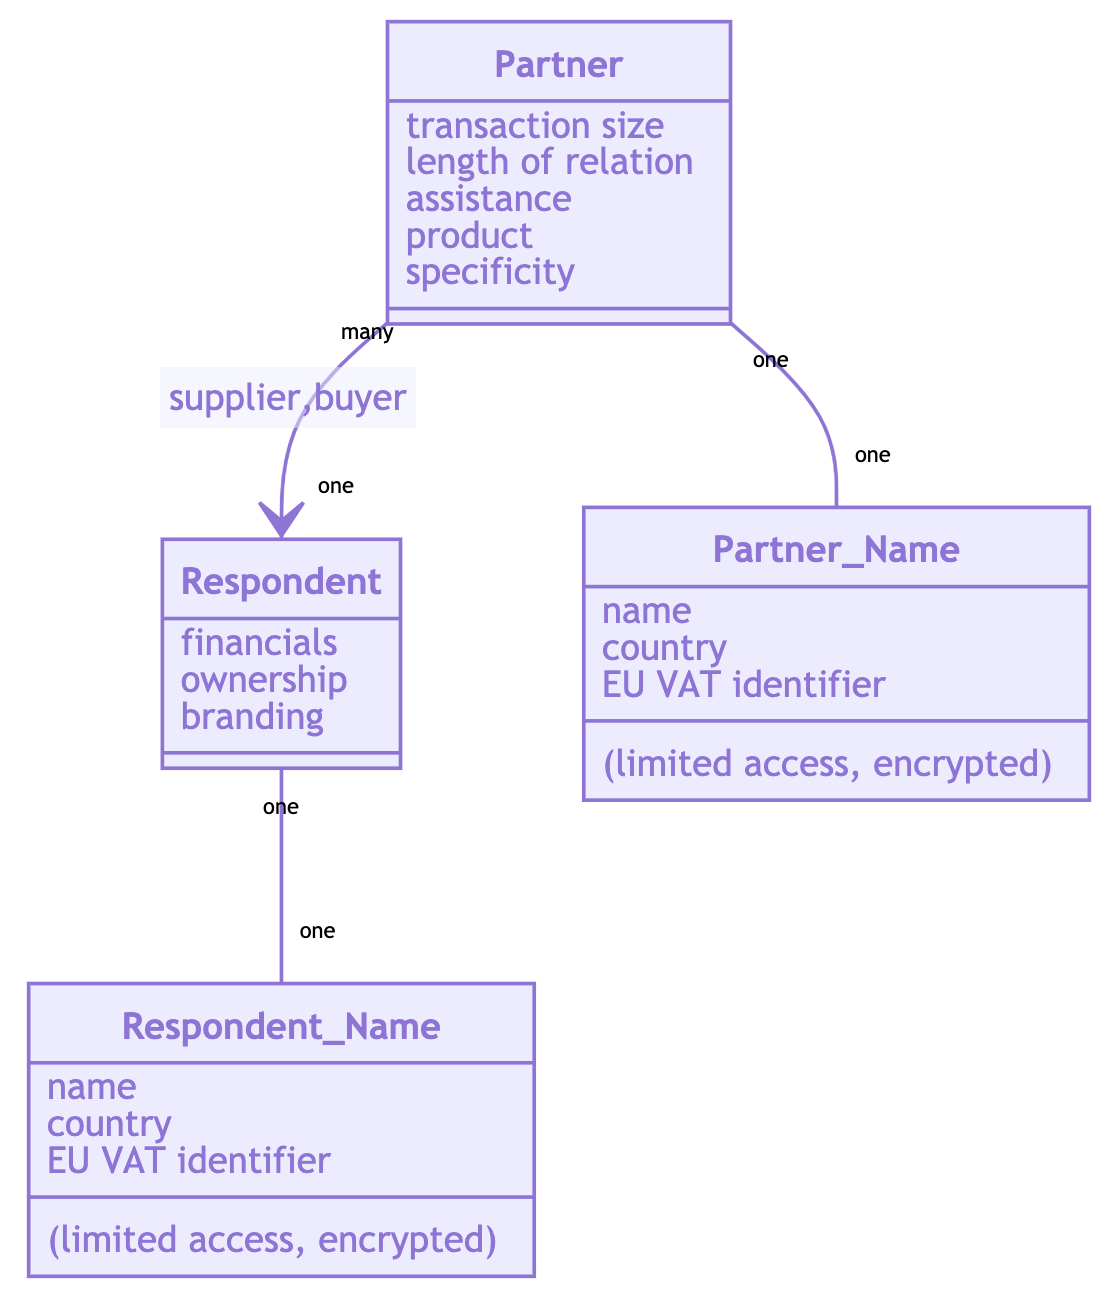
\includegraphics[width=0.7\textwidth]{graphs/ERD.png}
     \end{center}    
        {\scriptsize \textit{Notes:} This Figure shows the Entity-Relation Diagram of our analysis dataset. Each respondent can have multiple partners reported. The names of respondents and partners have been separated out in tables and handled separately to preserve anonymity. The graph gives a sample of information known about each entity, not a full list of variables.} 
\end{figure}

\subsection{Data security} 

As we have discussed in Subsection \ref{sec:trust}, data protection and security is key when conducting a survey about sensitive business information. In line with our Data Protection and Privacy Policy, we developed a data work flow accordingly. In particular, all information on company names and other identifiable information were masked. In addition, we checked variables and cleared names from text (sometimes firm names were mentioned in other free text questions).

Complying with our Policy and to protect against accidental data leakage, all privately identifiable information resides on encrypted media on electronically and physically protected servers on CEU premises. Only designated researchers have access to the privately identifiable data when doing data cleaning, for example. All other researchers have only access to anonymized data, also stored on encrypted devices.


\subsection{Harmonization} 

Surveys were very consistent across countries, therefore relatively little data cleaning was necessary. The main steps were the following:

\begin{enumerate}
    \item All values given in national currency or a currency the company used (could be USD). To harmonize this, they were converted to 1,000 EUR. 
    
    \item We corrected partner index numbering to ensure that the largest customer is indeed the one with the largest share (as some respondents mentioned their second largest customer first). We created a new share rank variable with correct ordering and values only for observations with non-missing shares. We added a flag when share was missing. This change affected about 3-4\% of rankings (for both domains, buyers and sellers). 
    
    \item We checked if shares satisfied basic algebraic constraints, such as being less than 100\% and summing up to less than 100\%. While some shares could have been erroneous, we saw no patterns suggesting intervention.
    
    \item We corrected every type of duplication based on partner information. The ``special'' buyer/supplier mentioned by the respondent was sometimes the same as one already described between the most important ones. We cleaned this by getting rid of duplicates. We used the key information on firms to find potential duplicates but also checked some cases by hand. This affected less than 5\% of observations.

\end{enumerate}

\subsection{Survey quality test}
\label{sec:quality_test}

%It is rather hard to check if surveyor features would effect results, actually. As regions and firms in these regions vary, replies to questions may vary across respondents. Furthermore, surveyors vary in experience and hence response time may vary for completely honest reasons, too. 


To study the quality of responses, we conducted several checks. We looked for correlations between quality of the survey data and metadata. Data quality can be captured by item non-response: how many questions remain unanswered on the questionnaire. Survey metadata includes an anonymous identifier of the surveyor and the precise time stamp of starting and completing the survey. These were recorded in the survey application, as all interviews were computer aided. 

We identified several surveyors who were very different from the vast majority in terms of the number of interviews conducted (too many), the time gap between surveys (too short), or the length of the interview (too short). However, interviews conducted by these surveyors did not differ significantly in terms of data quality indicators such as the prevalence of item nonresponse. We could not rule out that these interviews were, in fact, conducted in the same fashion as others, with data entry into the survey application happening at a later stage.

%% Gergo pls check language here

%%%%%%%%%%%%%%%%%%%%%%%%%%%%%%%%%%%%%%%
\section{Results of the survey}
\label{sec:desc}
%%%%%%%%%%%%%%%%%%%%%%%%%%%%%%%%%%%%%%%

In this section, we will present key results on buyer and supplier relationships. To conserve space, we mostly present results only for customers and note is the patterns are substantially different in the case of suppliers. When possible, we report the numbers separately for each country. We also show differences between different types of firms. When constructing firm groups there is a clear trade-off between presenting a large number of groups and having a decent number of observations in each group. As a compromise, we will classify firms into three groups: (i) Small domestic (below 51 employees), (ii) Large domestic and (iii) Foreign. 


%Define key suppliers if not done before

\subsection{Sample}


A first view of the data is presented by Table \ref{tab:obs}, which shows the number of observations along several dimensions. There are 1535 firms in the final sample, with 556 from Hungary, 584 from Romania and 395 from Slovakia. The majority of firms are small, with almost two thirds having less than 50 employees. This distribution is similar across countries, with large firms having a relatively larger share in Slovakia.

%%The percentages by size do not add up

The vast majority, 72\% of the firms in our sample are domestically owned and 28\% are foreign owned. These shares are also similar in the three countries, with a somewhat higher share of foreign-owned firms (37\%) in Slovakia. In terms of industry, the largest share of firms operate in the fabricated metals industry, followed by rubber/plastic and machinery.

%%%Any numbers from amadeus for the full population of firms?



\begin{table}[H]
\caption{Summary of firms by number of employees, ownership and industry}
\label{tab:obs}
\centerline{
%    
\begin{tabular}{lccc|c} 
\toprule
	Country		\\
	&Hungary	&Romania & Slovakia & Total \\
	&No. &No. &No. & \% \\
	\midrule
\ul{Number of employees}	&&&& \\			
Less than 20 &	203	&213&	179&	38.7\% \\
Between 21 and 50&	134&	167&	93	& 25.7\%\\
Between 51 and 250	&184	&167	&80	& 28.1\% \\
More than 250	&35&	37&	43	& 7.5\% \\
&&&&& \\
\ul{Ownership} &&&& \\				
Domestic	&409	&443	&249	& 71.7\% \\
Foreign	&147	&141	&146	& 28.3\% \\
&&&&& \\
\ul{Manufacturing sector} &&&&\\				
Chemicals & 	19 &	25 &	17	& 4\% \\
Pharmaceuticals&	3	&6	&4	& 0.85\% \\
Rubber and plastic &	67&	79&	50&	12.8\%\\
Non-metallic mineral&	37&	68&	35&	9.1\% \\
Basic metals	&13	&19	&7	& 2.5\%\\
Fabricated metals &	249	&235	&121&	39.4\%\\
Computer, electronic and optical &	24	&23&	27&	4.8\% \\
Electrical equipment	&36	&28	&42	& 6.9\% \\
Machinery &77	&60&	46&	11.9\%\\
Motor vehicles&	26&	24&	26&	4.6\%\\
Other transport equip. &	5	&17	&20	& 2.7\% \\
\midrule

Total	&556	&584	&395	& 100\% \\
\bottomrule
\end{tabular}
 
    
\begin{tabular}{lccc} 
\toprule
	Country		\\
	&Hungary	&Romania & Slovakia  \\
	\midrule
\ul{Number of employees}	&&& \\			
Less than 20 (38.7\%)	 &	203	&213&	179	 \\
Between 21 and 50  (25.7\%)	&	134&	167&	93	\\
Between 51 and 250 (28.1\%)		&184	&167	&80	  \\
More than 250	 (7.5\%)	&35&	37&	43	 \\
\addlinespace[2ex]
\ul{Ownership} &&& \\				
Domestic (71.7\%)	& 409	&443	&249	 \\
Foreign	 (28.3\%)	&147	&141	&146	 \\
\addlinespace[2ex]
\ul{Manufacturing sector} &&&\\				
Chemicals  (4\%)	& 	19 &	25 &	17	 \\
Pharmaceuticals (0.8\%)	&	3	&6	&4	 \\
Rubber and plastic  (12.8\%)	&	67&	79&	50\\
Non-metallic mineral  (9.1\%)	&	37&	68&	35 \\
Basic metals  (2.5\%)		&13	&19	&7	\\
Fabricated metals  (39.4\%)	&	249	&235	&121\\
Computer, electronic and optical (4.8\%)	 &	24	&23&	27 \\
Electrical equipment (6.9\%)		&36	&28	&42	\\
Machinery (11.9\%)	 &77	&60&	46 \\
Motor vehicles (4.6\%)	&	26&	24&	26 \\
Other transport equip. (2.7\%)	 &	5	&17	&20 \\
\midrule

Total	 (100\%)	&556	&584	&395	\\
\bottomrule
\end{tabular}
 
}
{\scriptsize \textit{Source: Central European Supplier Survey. Manufacturing sectors are NACE 1.1 2-digit categories. Ownership is based on majority owner. Number of employees is based on survey response}}
\end{table}


\subsection{Portfolios of buyers and suppliers}

Let us start with providing a picture about the number and distribution of suppliers and buyers (Table \ref{tab:num_supp}). 

Consider fist the median number of partners, presented in the third column. A robust insight is that these manufacturing firms tend to have significantly more buyers (30 in all three countries) than suppliers (between 10 and 20). This likely reflects that many of the smaller buyers are outside manufacturing, and clearly suggest an important asymmetry in the structure of the network. 

%% Slovakia supplier return share: 100% --> TO BE CHECKED

\begin{table}[H]
    \caption{Buyer and supplier portfolios (medians)}
    \label{tab:num_supp}
    \centerline{
    
\begin{tabular}{cccccc}
\hline
    Country & Buyer/Supplier & Number & \multicolumn{2}{c}{From which (\%):} & Length \\
     & & & Returning & TOP3 & \\
     &&&(number share) & (value share) & \\
     \hline
     Hungary  & buyer & 30 & 66.6\% & 47 &10 \\
              & supplier & 18 & 83.3\% & 40 &10 \\ 
     Romania  & buyer & 30 & 66.6\% & 60 &7 \\
              & supplier & 20 & 75\% & 59 &8 \\
     Slovakia & buyer & 30 & 40\% & 40 &6 \\
              & supplier & 10 & 100\% & 43.5 &7 \\ \hline
\end{tabular}
}
    {\scriptsize \textit{Notes:} This table shows firm-level median for the number of buyers, suppliers, the share of returning partners, the share of the TOP3 partners in sales/material costs, and the average length of key relationships. \textit{Source}: Central European Supplier Survey.}
\end{table}


Figure \ref{fig:kernel} zooms in by showing the full distribution of the number of customers. The shape of these log-transformed distributions suggest that the original distribution is fat-tailed, with a few firms having a very large number of partners while many firms having a small number of partners. Panel A of the Figure distinguishes between small domestic (less than 51 employees), larger domestic and foreign firms. While the shape of the distribution is similar for the three groups of firms, larger firms clearly tend to have more customers. Panel B shows the distribution for different countries. The figure suggests that not only the central tendency of the distributions (as Table \ref{tab:num_supp} has already shown) but also the whole shape of the distributions are very similar across countries.


\begin{figure}[h]    
    \begin{center}
    \caption{Kernel densities of the number of buyers}
    \label{fig:kernel}       
    \subfloat[By firm type]{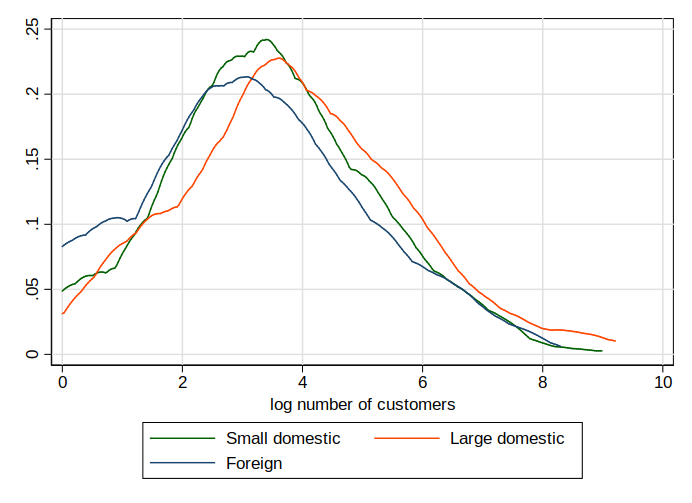
\includegraphics[width=7 cm]{graphs/Fig5a.png}}
    \subfloat[By country]{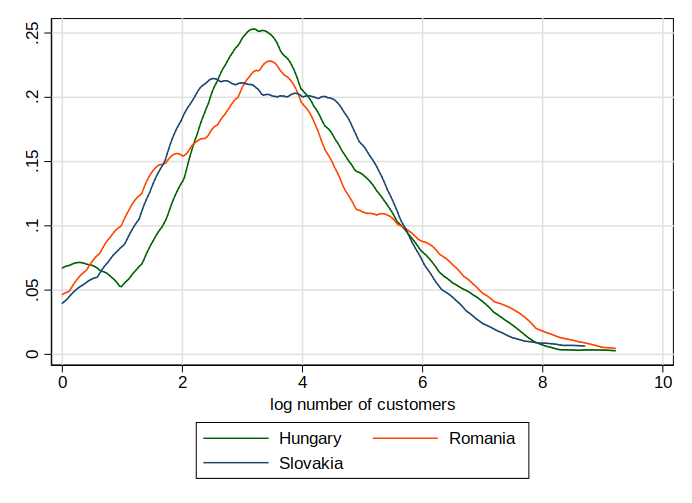
\includegraphics[width= 7cm]{graphs/Fig5b.png}}
    \end{center}
    {\footnotesize \textit{Notes:} This Figure shows kernel densities of the natural logarithm of the number of buyers. Small: $< 51$ employees, large otherwise. Foreign: foreign controlled. \textit{Source}: Central European Supplier Survey.}
\end{figure}


The fourth column of Table \ref{tab:num_supp} shows the median share of returning partners (``had bought from /sold to your company previously?''). Repeated or longer term relationships seem to be the norm rather than the exception for these firms. In Hungary, for example,  two thirds of the buyers were returning while more than 80\% of suppliers were returning for the typical firm. This also implies that manufacturing firms' relationships with their suppliers are slightly more likely to be repeated than their relationship with their buyers.

The fifth column of Table \ref{tab:num_supp} shows that supplier and buyer portfolios of manufacturing firms are quite concentrated. The largest three partners represent between 40\% and 60\% of sales or purchases for the typical firm. This concentration is high when compared to the typical number of partners. We do not find pronounced differences between the concentration of buyers and suppliers, and these shares are similar across countries.

Finally, the last column of Table \ref{tab:num_supp} shows the length of key relationships.\footnote{Recall that this question was only asked for key relationships.} We find that key relationships tend to be relatively old, between 6 and 10 years for the median firm. The longevity of key supplier and buyer relationships appear to be similar. There are pronounced country differences in this respect, with relationships being about 3 years longer in Hungary compared to the other two countries. 

While Table \ref{tab:num_supp} presented the central tendencies of the different variables, the survey data also allows us to analyze firm heterogeneity in these dimensions. Figure \ref{fig:happy_few} shows the inverse cumulative distribution functions of several variables. Panel A shows the distribution in the number of customers. In line with the patterns in Figure \ref{fig:kernel}, the distribution is skewed, the median firm having 30 customers and the 99th percentile being 400.

There are also substantial differences across firms in terms of the share of their new (non-returning) customers. 40\% of firms served only returning customers in 2015, while 20\% of firms had a share of new customers above 50\%. This pattern reinforces our earlier conclusion that longer-term relationships are the rule rather than the exception, but it also adds to the picture by showing that different firms face large differences in the share of their longer-term relationships.

The different strategic situation of firms is even more pronounced when we consider the concentration of their buyers. The top 3 buyers of the median firm are responsible for about half of the sales, but the share of top 3 buyers is above 80\% for 23.5\% of firms. This suggests that most firms face at least some buyers with a large power, but a substantial share of firms depend strongly on decisions of a few firms.

\newgeometry{top=4cm}
\begin{figure}[!h]
    \caption{Differences between customer portfolios}
    \label{fig:happy_few}
    \begin{center}
    \subfloat[Number of customers]{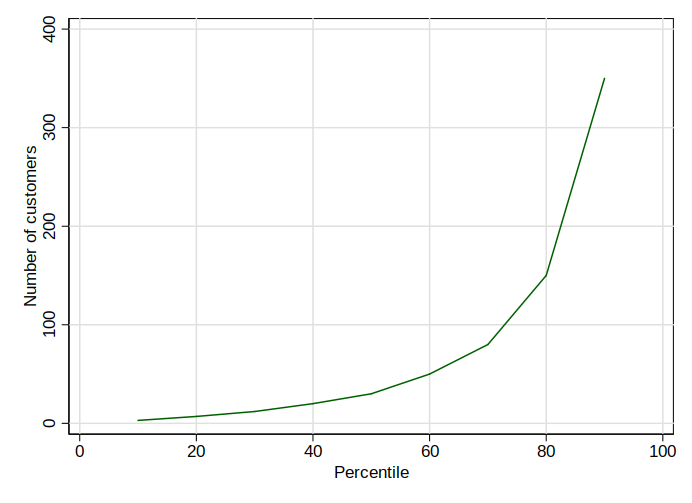
\includegraphics[width=7cm]{graphs/Fig4a.png}}
    \subfloat[Share of new customers]{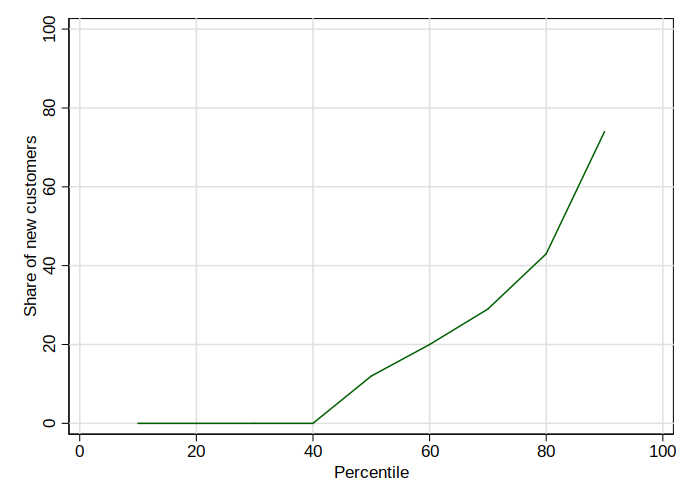
\includegraphics[width=7cm]{graphs/Fig4b.png}}\\
    \subfloat[Share of top customer]{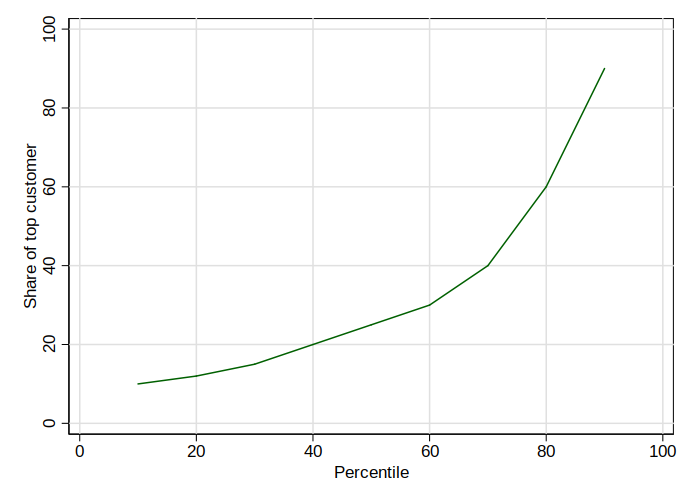
\includegraphics[width=7cm]{graphs/Fig4c.png}}
    \subfloat[Share of top 3 customers]{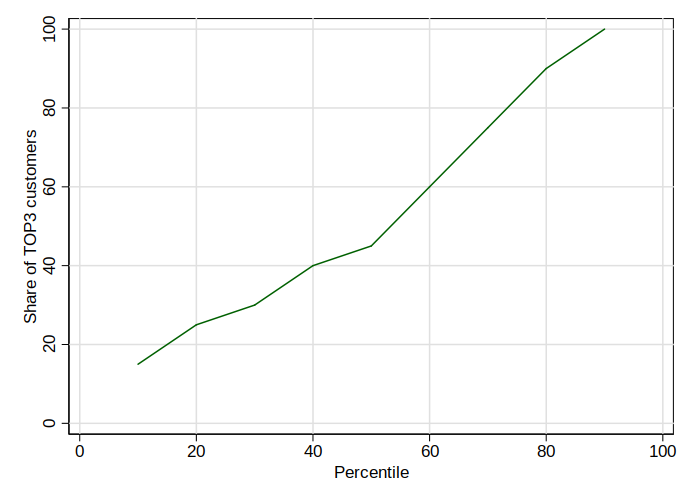
\includegraphics[width=7cm]{graphs/Fig4d.png}}
    \end{center}    
        {\footnotesize \textit{Notes:} This Figure shows the percentages (1-99) of the distribution of the above variables. \textit{Source}: Central European Supplier Survey.} 
\end{figure}
\restoregeometry

To sum up, we find that the supplier-buyer relationships of manufacturing firms are far from being atomized and short-term. A large share of partners are returning and the length of key relationships can easily be above 8-10 years. Buyer and supplier power seem to be substantial, with the top 3 partners typically responsible for more than half of sales or purchases. The survey also shows that there is a substantial amount of heterogeneity across firms in terms of how long-term their relationships are and how concentrated their buyer and supplier portfolio is. These facts imply that building supplier/buyer relationships are important strategic choices and may be strongly related to competitiveness.


\subsection{Supplier and buyer portfolios and performance}

In this subsection we conduct a simple analysis to see whether the quantity and quality of suppliers is associated with firm performance. To do so, we run regressions at the firm level with labor productivity as the dependent variable and measures of the buyer/supplier portfolio as explanatory variables. In particular, we run the following regression
%
\begin{equation}
    LP_{i|cjs}=\beta' X_{i}+\gamma \ln \text{employees}_i+\eta_c+\theta_j+\delta_s+u_i,
\end{equation}{}
%
where $i$ denotes firms, $c$ countries, $j$ 2-digit industries and $s$ size categories, $X_{i}$ is the vector of the variables of interest, and $\eta_c$, $\theta_j$ and $\delta_s$ are sets of country, industry and size category dummies, respectively. 

This strategy identifies from comparing firms in the same country, industry and size category but with different buyer and supplier structure. Naturally, in this cross sectional regression many key firm variables remain unobserved, therefore the results should be interpreted as suggestive correlations rather than causal effects. Although we focused on variables with good coverage, some buyer/supplier information is not available for all the firms in our sample. As a result, the sample for this exercise is 1129 firms (73\% of the 1535 firms in the survey). 

%BG LP is computed from survey or amadeus? If amadeus, then we also lose bc missing sales. 

Table \ref{tab:prod_regs} presents the results of these regressions. In column (1) only the $\ln$ number of buyers and suppliers are included in addition to the base firm controls. We find that the number of suppliers (but not that of buyers) is strongly correlated with labor productivity. A firm having twice as many suppliers will have 4.2\% higher productivity levels. The sign of the controls variables are as expected: larger firms and members of business groups are more productive.

In column (2) we start to control for the type of partners the firm has. First, we ask whether having at least one buyer and/or supplier from the firm's business group matters for productivity. We find a strong relationship between productivity and the presence of \textit{buyers} from the business group: firms having at least one such buyer tend to be more productive by 13\%.\footnote{Note that we already control for whether the firm itself is a member of the business groups, therefore this coefficient captures the additional effect of having buyers from the same group.} Column (2) does not show evidence for an association between having foreign buyers or sellers and productivity. In column (3) we also include the average length of the relationship with key buyers and suppliers.\footnote{Note that this reduces the sample to firms which have named key partners and also reported the duration of those relationships.} These variables are not significant.

To sum up, the portfolio of buyers and supplier is actually correlated with firm performance. In particular, labor productivity is associated with the number of suppliers a firm has and also whether some of the buyers are from the same business group. There results underline that partner portfolios are related to performance and therefore being more successful in building such portfolios may generate a competitive advantage.


\begin{table}[H]
    \caption{Labor productivity and supplier/buyer characteristics}
    \label{tab:prod_regs}
    \centerline{
\begin{tabular}{lccc} \hline
 & (1) & (2) & (3) \\
VARIABLES & LP & LP & LP \\ \hline
 &  &  &  \\
ln(Number of buyers) & 0.014 & 0.021 & 0.016 \\
 & (0.013) & (0.014) & (0.015) \\
ln(Number of suppliers) & 0.059*** & 0.057*** & 0.069*** \\
 & (0.017) & (0.017) & (0.019) \\
Has buyer from business group &  & 0.137** & 0.155** \\
 &  & (0.057) & (0.061) \\
Has supplier from business group &  & -0.073 & -0.050 \\
 &  & (0.060) & (0.064) \\
Has foreign buyer &  & 0.023 & 0.035 \\
 &  & (0.051) & (0.057) \\
Has foreign supplier &  & -0.081 & -0.056 \\
 &  & (0.050) & (0.058) \\
Mean relationship length, buyers &  &  & 0.007 \\
 &  &  & (0.005) \\
Mean relationship length, sellers &  &  & -0.005 \\
 &  &  & (0.005) \\
ln(Employment) & 0.110*** & 0.104*** & 0.097*** \\
 & (0.025) & (0.026) & (0.028) \\
Group member & 0.161*** & 0.140*** & 0.136** \\
 & (0.049) & (0.052) & (0.057) \\
\hline
Country, sector, size dummies &YES &YES &YES\\
Observations & 1,129 & 1,129 & 996 \\
 R-squared & 0.325 & 0.330 & 0.339 \\ \hline
\end{tabular}

}

    {\scriptsize \textit{Notes:} The table shows OLS regressions when the dependent variable is ln(labor productivity). One observation is one respondent. Business group and foreign refers to whether the firm has at least one such partner, while length is the average length of key relationships. Standard errors in parentheses$ *** p$<$0.01, ** p$<$0.05, * p$<$0.1 $. \textit{Source}: Central European Supplier Survey.}
\end{table}
    

\subsection{Starting relationships}

After showing that performance is related to the number and type of buyers of the firm, we ask how these relationships form. What do firms do to build a portfolio which can support high performance more effectively?

In our questionnaire we asked how each key relationship had formed. Based on the answer to that question we can distinguish between four main types of relationship formation: (i) supplier initiated; (ii) buyer initiated; (iii) within groups and (iv) other ways (including professional events and networking). 

The results are presented in Figure \ref{fig:rel_form}. Buyer and supplier initiated relationships are similarly prevalent, representing more than half of all relationships. Intra-group relationships are especially important in the case of foreign firm, where 36\% of key buyers are from the same business group. Slightly more than 30\% of key relationships formed via networking, professional events and in other ways. 
%here i am

These patterns are similar across countries, with within-group relationships playing a somewhat smaller role in Hungary compared to the other two countries. Another difference is that supplier initiated key relationships substantially outnumber buyer initiated ones in Romania, while the two sides initiate to a more similar extent in Hungary and Slovakia.

A number of conclusions can be drawn from these patterns. First, the searching process is clearly two-sided, and presumably many relationship require substantial investments from both sides. Therefore finding buyers does not only require investments from the supplier. Second, within-group relationships represent a substantial share of important relationships, especially for foreign firms. Understanding multinational groups is important when describing the empirically observed supplier-buyer networks. Third, while a substantial number of relationships are created by networking and at professional events, the majority of relationships form besides these platforms. Policymakers aiming at promoting the creation of high-value relationships may use policy instruments that go beyond organizing such events. 

\begin{figure}[h]    
    \begin{center}
    \caption{How do firms find customers?}  
    \label{fig:rel_form}       
    \subfloat[By country]
    {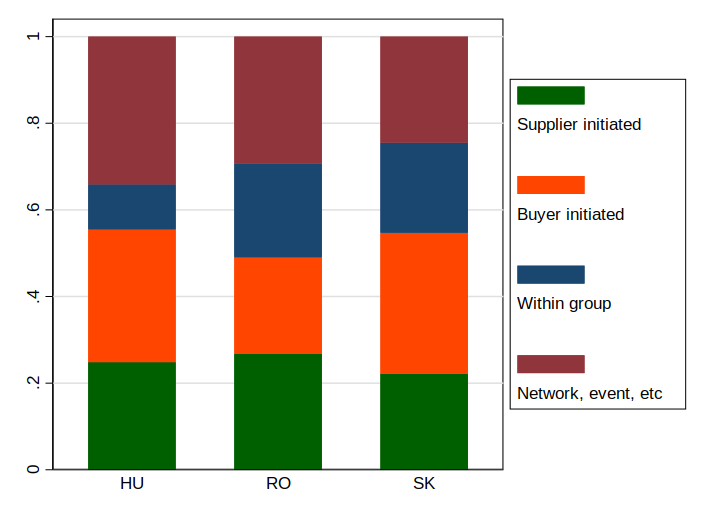
\includegraphics[width=7cm]{graphs/Table6a.png}}
    \subfloat[By firm type]
    {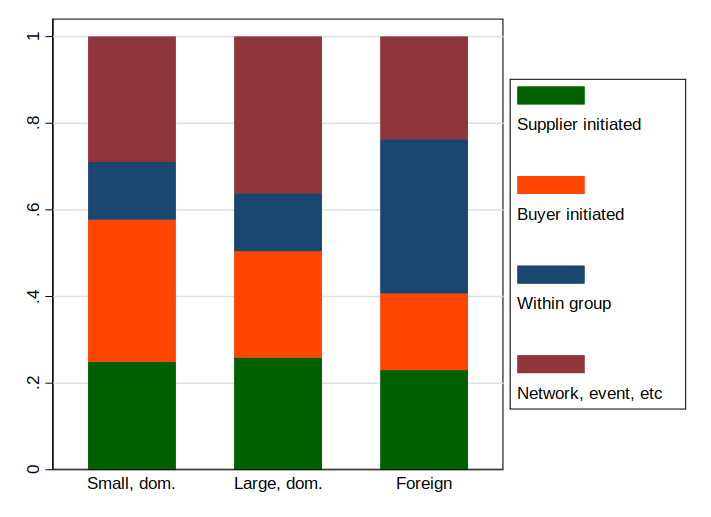
\includegraphics[width=7cm]{graphs/Table6b.png}}
    \end{center}
    {\footnotesize \textit{Notes:} The figure shows the distribution of the answers to ``How did the relationship start?'' for key relationships (each such relationship when respondent is supplier is one observation). }     
\end{figure}

While search is clearly a key element of new relationship formation, establishing the relationship often requires even more substantial investments. Figure \ref{fig:innov} shows the share of key relationships which started with product innovation, process innovation or both. We find that a large share of relationships indeed begin with innovation, though differences across countries are also substantial: 47.5\% in Hungary, 22.2\% in Romania and 40.4\% in Slovakia. Interestingly, product and process innovations appear to be strongly complementary: the majority of innovators conduct both types of innovation. Only modifying the product for the demands of the buyer may not be enough - the revamping of the production process is often necessary.


Panel B of Figure \ref{fig:innov} distinguishes between firms types. We find that larger and foreign owned firms are more likely to innovate when starting key relationships compared to small domestically owned ones. This interesting pattern suggests that innovation is not something less productive firms do to upgrade their technological level when starting to supply an important partner, but it is an activity which allows more productive firms personalize to their processes and products to fit better their important potential buyers. This 'innovation gap' may be an additional reason for smaller firms being less able to serve large and productive partners. Not only their technology level but also their innovation capabilities may lag behind that of more productive firms. 

    
 \begin{figure}[h]    
    \begin{center}
    \caption{Innovation when relationship starts}  
     \label{fig:innov}
    \subfloat[By country]
    {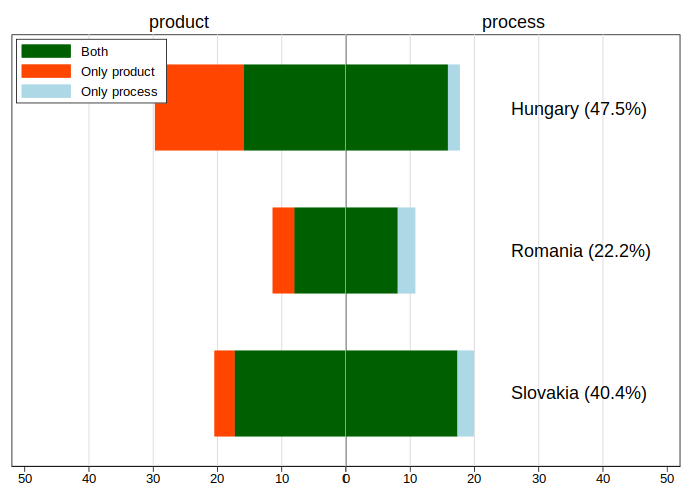
\includegraphics[width=7cm]{graphs/Fig7a.png}}
    \subfloat[By size and ownership]
    {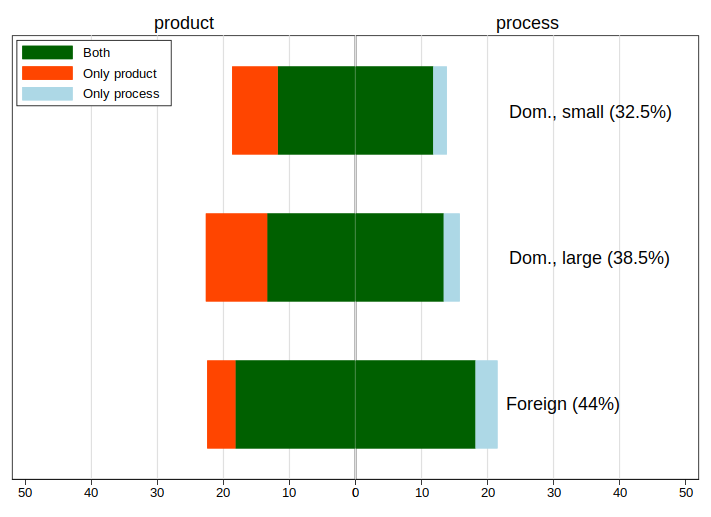
\includegraphics[width=7cm]{graphs/Fig7b.png}}
    \end{center}
    {\footnotesize \textit{Notes:} The figure shows the distribution of the answers to ’did the firm have to improve its product/process for the relationship at the beginning’ for key relationships (each such relationship when respondent is supplier is one observation). \textit{Source}: Central European Supplier Survey.}}     
\end{figure}   
    
Investing into a relationship, however, is not a lonely activity. Suppliers' Innovation is in fact often supported by the buyer. Table \ref{tab:start_support} shows the type of support from the buyer to the supplier at the start of the relationship, according to the supplier. The table distinguishes between between different types of suppliers and buyers. The questionnaire distinguished between three types of support: (i) technology transfer, (ii) asset transfer and (iii) regular consulting, meeting.

The most frequent type of support involves regular meetings (28.2\%), followed by technology transfer (17.5\%) and asset transfer (7.8\%). Buyers, especially domestic ones, often provide assistance for product development: consulting in 1/4, technology transfer in 1/8 and asset transfer in 1/16 of key relationships.


\begin{table}[h]
    \caption{Support for product innovation from customers at the start of the relationship}
    \label{tab:start_support}
    
\begin{tabular}{lcccc} \hline
Type of customer	&\multicolumn{4}{c}{Type of reporting firm (seller)}	\\		
	&Domestic SME	&Domestic large	&Foreign-owned	&Total \\
	\hline
	\hline
&\multicolumn{4}{c}{Technology transfer}\\
Domestic SME	&18.1	&100.0	&63.6	&21.0 \\
Domestic large	&25.2	&25.9	&25.7	&25.3
Abroad	&13.0	&27.1	&20.7	&13.7\\
Total	&16.4	&27.8	&26.2	&17.5\\
\hline	
	
&\multicolumn{4}{c}{Asset transfer}\\
Domestic SME&	6.9&	0.0&	63.6&	9.6\\
Domestic large&	15.0&	11.1&	15.8&	14.9\\
Abroad&	4.2&	8.6&	10.3&	4.5\\
Total&	7.1&	9.5&	16.7&	7.8\\
\hline
&\multicolumn{4}{c}{Regular meetings, consulting}\\
Domestic SME&	24.5&	50.0&	54.5&	26.2\\
Domestic large&	39.0&	27.8&	34.5&	37.6\\
Abroad&	23.9&	31.4&	29.3&	24.3\\
Total&	27.7&	30.2&	34.2&	28.2\\
\hline
\end{tabular}



    {\scriptsize \textit{Notes:} The table shows the fraction of firms who responded having received a specific type of assistance from its buyer for product development at the start of the relationship. Buyer-supplier relationships are grouped by firm type. Only key relationships included. SME: $\le 50$ employees, large otherwise. \textit{Source}: Central European Supplier Survey.}}
\end{table}

Our main findings about relationship formation can be summarized as follows. First, searching and starting relationships is a two sided process: often both parties invest heavily into searching for partners and establishing relationships. Second, starting key relationships requires innovation, often both by modifying products and processes. Such innovations are more likely to be undertaken by more productive firms, showing that these are specific investments rather than general technology upgrades for firms with low productivity levels. The innovations often involve some form of cooperation between the buyer and supplier, suggesting that co-innovation plays an important part. All these patterns, together with the longevity of these relationships suggest that many of the key supplier-buyer contacts are relational rather than simply market-based. 

\section{Summary and discussion}
\label{sec:conclusions}
We conducted a survey of buyer-supplier linkages in a sample of manufacturing firms in Hungary, Romania and Slovakia. We discussed the key design and implementation choices for the Central European Supplier Survey and provided explorative analysis of firm responses about their business partners.

There are broad patterns of business link formation that are similar across countries and industries. Most manufacturing firms have more buyers than suppliers and bigger firms have more of each type of partner. A very small fraction of business partners capture a large share of revenue and cost for most firms. This degree of concentration suggests that buyer-seller networks provide an important structural constraint to firm strategy. Many firms have a potentially unbalanced power relation with much larger business partners. It hence seems important to study how firms can diversify the portfolio of their buyers and sellers.

Regarding the formation of relationships we found that this is a two-sided process. Buyers and suppliers are similarly likely to initiate the relationship, suggesting a two-way search process. On the supplier side, starting the relationship requires an innovation effort, often involving both product and process innovation. This, however, is often supported by the buyer, mostly by technical advice, but also with technology or asset transfer in a number of cases.

The most important benefit of our survey is that it can tease out qualitative information about business relationships, which are difficult to collect in observational data. We hence view this methodology complementary to collecting large-scale administrative datasets about business-to-business transactions (such as from VAT filings). To understand the long-term stability and success of business relationships, we need to have much more information than just the volume of transactions, which is typically the only metric available in transactional data. Well-designed surveys can elicit information about the length of the relationship, the steps each party has taken to form and maintain the relationship, the flow of information and assistance in the relationship and other qualitative indicators measuring the relative market power of each partner.

We see a number of direct applications of the Central European Supplier Survey and the methodology we accumulated. First, we can study the role of geography and other frictions in forming buyer-supplier links. Our preliminary analysis suggests that suppliers are located closer to buyers than random firms in the same industry. This may be natural, but the exact ways in which geography affects link formation is not known. Second, given the collected information about the formation of a business link, we can ask what it takes for domestic firms to join GVCs. What are the characteristics of firms that sell to multinational business groups and what steps did they take to link up with their buyer? Third, it is interesting how communication and the flow of knowledge and technology can maintain the relation in the long run. Many suppliers receive assistance from their buyers, but the exact nature of this assistance and its role in the longevity of the buyer-supplier relation should be studied further. Fourth, our survey and similar studies can inform about the power balance in GVCs and the transmission of economic shocks. For example, our previous survey (\cite{still_standing}) found that local firms at the bottom of a GVC were hit harder by the great recession than headquarter firms at the top of the GVC. Studying the buyer-supplier relationship more directly can shed light on this question and other policy debates.

\section{References}

\bibliographystyle{agsm}
\bibliography{biblio}

\appendix
\section{Appendix}

\end{document}
